\documentclass[]{article}
\usepackage{lmodern}
\usepackage{amssymb,amsmath}
\usepackage{ifxetex,ifluatex}
\usepackage{fixltx2e} % provides \textsubscript
\ifnum 0\ifxetex 1\fi\ifluatex 1\fi=0 % if pdftex
  \usepackage[T1]{fontenc}
  \usepackage[utf8]{inputenc}
\else % if luatex or xelatex
  \ifxetex
    \usepackage{mathspec}
  \else
    \usepackage{fontspec}
  \fi
  \defaultfontfeatures{Ligatures=TeX,Scale=MatchLowercase}
\fi
% use upquote if available, for straight quotes in verbatim environments
\IfFileExists{upquote.sty}{\usepackage{upquote}}{}
% use microtype if available
\IfFileExists{microtype.sty}{%
\usepackage{microtype}
\UseMicrotypeSet[protrusion]{basicmath} % disable protrusion for tt fonts
}{}
\usepackage[margin=0.8in]{geometry}
\usepackage{hyperref}
\PassOptionsToPackage{usenames,dvipsnames}{color} % color is loaded by hyperref
\hypersetup{unicode=true,
            pdftitle={Canada glaciers trend analisys},
            pdfauthor={Stanislav},
            colorlinks=true,
            linkcolor=magenta,
            citecolor=Blue,
            urlcolor=blue,
            breaklinks=true}
\urlstyle{same}  % don't use monospace font for urls
\usepackage{longtable,booktabs}
\usepackage{graphicx,grffile}
\makeatletter
\def\maxwidth{\ifdim\Gin@nat@width>\linewidth\linewidth\else\Gin@nat@width\fi}
\def\maxheight{\ifdim\Gin@nat@height>\textheight\textheight\else\Gin@nat@height\fi}
\makeatother
% Scale images if necessary, so that they will not overflow the page
% margins by default, and it is still possible to overwrite the defaults
% using explicit options in \includegraphics[width, height, ...]{}
\setkeys{Gin}{width=\maxwidth,height=\maxheight,keepaspectratio}
\IfFileExists{parskip.sty}{%
\usepackage{parskip}
}{% else
\setlength{\parindent}{0pt}
\setlength{\parskip}{6pt plus 2pt minus 1pt}
}
\setlength{\emergencystretch}{3em}  % prevent overfull lines
\providecommand{\tightlist}{%
  \setlength{\itemsep}{0pt}\setlength{\parskip}{0pt}}
\setcounter{secnumdepth}{0}
% Redefines (sub)paragraphs to behave more like sections
\ifx\paragraph\undefined\else
\let\oldparagraph\paragraph
\renewcommand{\paragraph}[1]{\oldparagraph{#1}\mbox{}}
\fi
\ifx\subparagraph\undefined\else
\let\oldsubparagraph\subparagraph
\renewcommand{\subparagraph}[1]{\oldsubparagraph{#1}\mbox{}}
\fi

%%% Use protect on footnotes to avoid problems with footnotes in titles
\let\rmarkdownfootnote\footnote%
\def\footnote{\protect\rmarkdownfootnote}

%%% Change title format to be more compact
\usepackage{titling}

% Create subtitle command for use in maketitle
\providecommand{\subtitle}[1]{
  \posttitle{
    \begin{center}\large#1\end{center}
    }
}

\setlength{\droptitle}{-2em}

  \title{Canada glaciers trend analisys}
    \pretitle{\vspace{\droptitle}\centering\huge}
  \posttitle{\par}
    \author{Stanislav}
    \preauthor{\centering\large\emph}
  \postauthor{\par}
    \date{}
    \predate{}\postdate{}
  
\usepackage[T2A]{fontenc}
\usepackage[utf8]{inputenc}
\usepackage[russian]{babel}
\usepackage{caption}
\usepackage{subcaption}

\begin{document}
\maketitle

{
\hypersetup{linkcolor=black}
\setcounter{tocdepth}{2}
\tableofcontents
}
\subsection{Inroduction}\label{inroduction}

The data used in study is taken from:
\url{https://open.canada.ca}\footnote{\href{https://open.canada.ca/data/en/dataset/aca5e1de-c234-5372-b714-ae20300fb6ce}{Goverment
  of Canada site}}. The algorithm is taken from Antonov and Ermakov
(2015).

This data set contains 518 measurments of 6 Canadian glaciers mass
balance, collected from 1960 till 2007. Namely, the file includes these
glaciers:

\begin{verbatim}
## [1] "Devon Ice Cap NW - Devon Island, Nunavut"                                             
## [2] "Helm Glacier - southern Coast Mountains (Garibaldi Provincial Park), British Columbia"
## [3] "Meighen Ice Cap - Meighen Island, Nunavut"                                            
## [4] "Peyto Glacier - Rocky Mountain eastern slopes (Banff National Park), Alberta"         
## [5] "Place Glacier - southern Coast Mountains, British Columbia"                           
## [6] "White Glacier - Axel Heiberg Island, Nunavut"
\end{verbatim}

\subsection{Hypothesis}\label{hypothesis}

We are interested in finding out whether there is a statistically
significant change in mass balance over the observed time period.
purposes we use \textbf{R} (version 3.5.3) and an appropriate
statistical test called \emph{t-test}:
\[t = \frac{\overline{x} - \mu_0}{s/\sqrt{n]}}.\]

The workflow is as follows:

\begin{enumerate}
\def\labelenumi{\arabic{enumi}.}
\item
  \begin{quote}
  Read file
  \end{quote}
\item
  \href{Run\%20t-test\%20for\%20each\%20glacier\%20and\%20collect\%20p-values}{text}
\item
  \emph{Support the evidence with}
\end{enumerate}

\begin{itemize}
\tightlist
\item
  \textbf{a table of results;}
\item
  a plot the could help demonstrate the effect.
\end{itemize}

\begin{longtable}[]{@{}lrrrrrr@{}}
\caption{descriptive statistics}\tabularnewline
\toprule
Name & YearsObserved & MeanChange & WorstChange & WorstYear & Pvalue &
ConfidentLimit\tabularnewline
\midrule
\endfirsthead
\toprule
Name & YearsObserved & MeanChange & WorstChange & WorstYear & Pvalue &
ConfidentLimit\tabularnewline
\midrule
\endhead
Devon Ice Cap NW & 47 & -91.2 & -559 & 2001 & 5.81e-05 &
-39.0\tabularnewline
Helm Glacier & 31 & -1277.3 & -2850 & 1998 & 1.73e-07 &
-798.0\tabularnewline
Meighen Ice Cap & 48 & -107.6 & -970 & 1962 & 4.51e-03 &
-12.5\tabularnewline
Peyto Glacier & 42 & -579.9 & -2230 & 1998 & 3.62e-07 &
-339.7\tabularnewline
Place Glacier & 43 & -861.4 & -2486 & 1995 & 3.70e-09 &
-572.3\tabularnewline
White Glacier & 48 & -152.4 & -818 & 2007 & 6.56e-05 &
-64.3\tabularnewline
\bottomrule
\end{longtable}

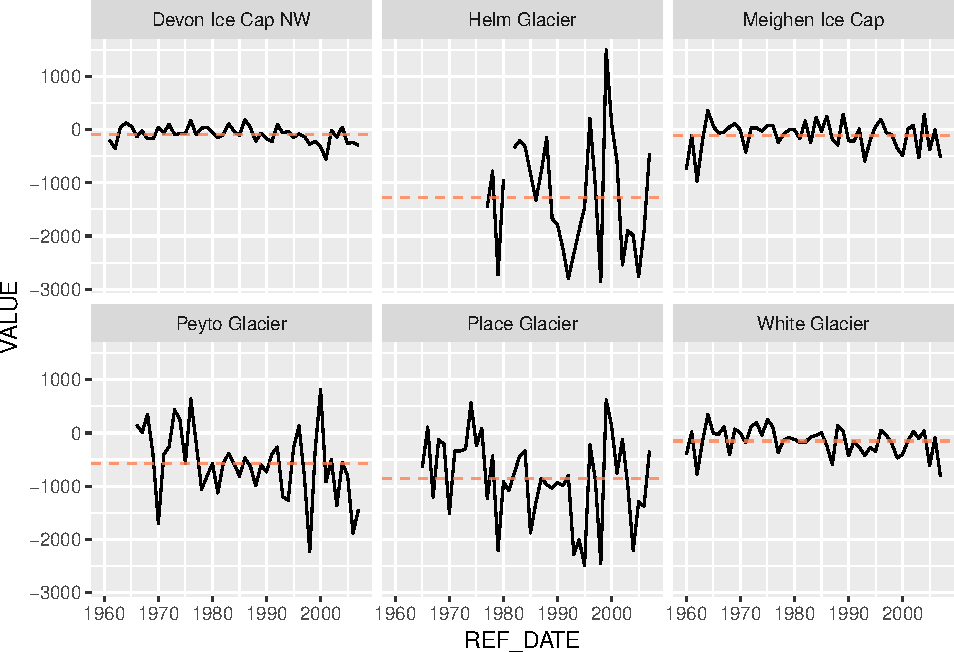
\includegraphics{R-3-Markdown_files/figure-latex/unnamed-chunk-4-1.pdf}

\subsection{Analisys}\label{analisys}

 првиет

\subsection*{Bibliography}\label{bibliography}
\addcontentsline{toc}{subsection}{Bibliography}

\hypertarget{refs}{}
\hypertarget{ref-AntonovErmakov_RandomCubaturesQMC}{}
Antonov, A.A., and S.M. Ermakov. 2015. ``Random Cubatures and
Quasi-Monte Carlo Methods.'' \emph{Monte Carlo Methods and Applications}
21 (3): 179--87.
doi:\href{https://doi.org/10.1515/mcma-2015-0102}{10.1515/mcma-2015-0102}.


\end{document}
